\documentclass[]{elsarticle} %review=doublespace preprint=single 5p=2 column
%%% Begin My package additions %%%%%%%%%%%%%%%%%%%

\usepackage[hyphens]{url}

  \journal{BioR\(\chi\)iv} % Sets Journal name

\usepackage{graphicx}
%%%%%%%%%%%%%%%% end my additions to header

\usepackage[T1]{fontenc}
\usepackage{lmodern}
\usepackage{amssymb,amsmath}
% TODO: Currently lineno needs to be loaded after amsmath because of conflict
% https://github.com/latex-lineno/lineno/issues/5
\usepackage{lineno} % add
\usepackage{ifxetex,ifluatex}
\usepackage{fixltx2e} % provides \textsubscript
% use upquote if available, for straight quotes in verbatim environments
\IfFileExists{upquote.sty}{\usepackage{upquote}}{}
\ifnum 0\ifxetex 1\fi\ifluatex 1\fi=0 % if pdftex
  \usepackage[utf8]{inputenc}
\else % if luatex or xelatex
  \usepackage{fontspec}
  \ifxetex
    \usepackage{xltxtra,xunicode}
  \fi
  \defaultfontfeatures{Mapping=tex-text,Scale=MatchLowercase}
  \newcommand{\euro}{€}
\fi
% use microtype if available
\IfFileExists{microtype.sty}{\usepackage{microtype}}{}
\usepackage[margin=1in]{geometry}
\usepackage[]{natbib}
\bibliographystyle{plainnat}

\ifxetex
  \usepackage[setpagesize=false, % page size defined by xetex
              unicode=false, % unicode breaks when used with xetex
              xetex]{hyperref}
\else
  \usepackage[unicode=true]{hyperref}
\fi
\hypersetup{breaklinks=true,
            bookmarks=true,
            pdfauthor={},
            pdftitle={The Quest for Dynamic Consistency --- A Comparison of OpenSim Tools for Residual Reduction in Simulations of Human Running},
            colorlinks=false,
            urlcolor=blue,
            linkcolor=magenta,
            pdfborder={0 0 0}}

\setcounter{secnumdepth}{0}
% Pandoc toggle for numbering sections (defaults to be off)
\setcounter{secnumdepth}{0}


% tightlist command for lists without linebreak
\providecommand{\tightlist}{%
  \setlength{\itemsep}{0pt}\setlength{\parskip}{0pt}}







\begin{document}


\begin{frontmatter}

  \title{The Quest for Dynamic Consistency --- A Comparison of OpenSim
Tools for Residual Reduction in Simulations of Human Running}
    \author[School of Exercise and Nutrition Sciences]{Aaron S. Fox%
  %
  \fnref{1}}
  
      \affiliation[School of Exercise and Nutrition Sciences]{School of
Exercise and Nutrition Sciences, Deakin University, Geelong, Australia}
    \cortext[cor1]{Corresponding author}
    \fntext[1]{Contact: aaron.f@deakin.edu.au}
  
  \begin{abstract}
  The use of synchronous kinematic and kinetic data in simulations of
  human running will typically lead to dynamic inconsistencies
  (i.e.~residual forces and moments) being present. Minimising the
  residual forces and moments in such simulations is important to ensure
  plausible model outputs (e.g.~joint moments, muscle forces) are
  obtained. A variety of approaches suitable for residual reduction are
  available in OpenSim, however a detailed comparison of these is yet to
  be conducted. This study compared a variety of OpenSim tools
  applicable for residual reduction in simulations of human running. A
  series of approaches (i.e.~singular and iterative Residual Reduction
  Algorithm, \emph{MocoTrack}, \emph{AddBiomechanics}) designed to
  reduce residual forces and moments were examined using an existing
  dataset of 10 male participants running on a treadmill at 5.0
  m·s\textsuperscript{-1} (\emph{n} = 3 gait cycles per participant).
  The computational time, resultant residual forces and moments, and
  output joint kinematics and kinetics from each approach were compared.
  A computational cost to residual reduction trade-off was identified,
  where lower residual forces and moments were achieved using approaches
  that required longer computational times. All of the tested approaches
  regularly reduced residual forces below recommended thresholds,
  however only the \emph{MocoTrack} approach could consistently achieve
  acceptable levels for residual moments. The \emph{AddBiomechanics} and
  \emph{MocoTrack} approaches produced variable lower and upper body
  kinematics, respectively, versus the remaining approaches; with
  minimal other qualitative differences were identified between joint
  kinematics from each approach. Joint kinetics were qualitatively
  similar between approaches, however \emph{MocoTrack} generated much
  noisier joint kinetic signals. The \emph{MocoTrack} approach was the
  most consistent and best performing approach for reducing residuals to
  near-zero levels, at the cost of longer computational times and
  potentially noisier joint kinetic signals. This study provides OpenSim
  users with evidence to inform decision-making at the residual
  reduction step of their modelling and simulation workflow when
  analysing human running.
  \end{abstract}
    \begin{keyword}
    biomechanics \sep musculoskeletal modelling \sep 
    gait
  \end{keyword}
  
 \end{frontmatter}

\hypertarget{introduction}{%
\section{Introduction}\label{introduction}}

Biomechanical data (i.e.~kinematics and kinetics) are commonly collected
and used alongside musculoskeletal models to understand human running
performance or injury risk. Kinematic data is typically collected via
marker-based optical motion capture systems, with kinetic data
synchronously collected via in-ground force plates or instrumented
treadmills. The independent measurement and associated error
(i.e.~noise) of kinematic and kinetic data in gait experiments leads to
dynamic inconsistencies in modelled data \citep{Hicks2015}. Residual
forces and moments at the `root' segment (i.e.~the segment connected to
the `ground' in a model --- typically the pelvis) remain present to
ensure dynamic consistency between the motion and external forces. The
presence of dynamic inconsistencies can lead to implausible conclusions
in simulation outputs (e.g.~joint moments, muscle forces) given that not
all of the forces are accounted for by realistic parts of the model. It
is therefore common practice for biomechanists to employ strategies that
minimise or eliminate residual forces and moments \citep{Hicks2015}.

~

Adjusting model parameters (e.g.~segment masses) and/or motion
(e.g.~joint kinematics) is a common approach for minimising residual
forces and moments in gait simulations \citep{Hicks2015, Werling2023}.
OpenSim is a widely used modelling and simulation software, and offers
the Residual Reduction Algorithm (RRA) as its main tool for minimising
dynamic inconsistencies between modelled motions and external forces
during gait \citep{Delp2007}. RRA employs a forward dynamics simulation
to adjust model kinematics and the mass centre of a selected body
(typically the torso), while also providing recommendations for
adjusting the mass of individual segments as a means to reduce residual
forces and moments \citep{NCSRR2017}. RRA can be effective in reducing
residuals within recommended thresholds \citep{Hicks2015}, however the
process is dependent on selecting tracking weights for joint coordinates
which may be difficult to objectively determine
\citep{Samaan2016, Sturdy2022}. Further, RRA has been employed as both a
singular \citep{Hamner2013} and iterative \citep{Rajagopal2016} process
--- yet there are no specific recommendations on which of these
approaches or how many iterations are optimal.

~

The expansion of OpenSim's toolkit in recent years offers potential
alternatives for generating dynamically consistent gait simulations.
OpenSim Moco \citep{Dembia2020} provides an option to leverage direct
collocation to achieve dynamic consistency --- using the
\emph{MocoTrack} class to generate torque-driven simulations that track
and adjust model kinematics, while minimising residual forces and
moments. The recently released \emph{AddBiomechanics} web application
\citep{Werling2023} aims to automate typical modelling processes
(i.e.~model scaling, inverse kinematics, inverse dynamics), and includes
an optimisation step that updates model segment masses and joint
kinematics to minimise dynamic inconsistencies in the final simulation
results. A detailed comparison of available tools and their capacity to
achieve dynamically consistent simulations of human running can provide
researchers with information on which may be the most suitable
approach(es). The purpose, nay quest, of this study was to compare the
various OpenSim tools available for residual reduction in simulations of
human running, with particular reference to the: (i) computational time;
(ii) resultant residual forces and moments; and (iii) output joint
kinematics and kinetics of each approach.

\hypertarget{methods}{%
\section{Methods}\label{methods}}

\hypertarget{dataset}{%
\subsection{Dataset}\label{dataset}}

This study used the human running dataset provided by Hamner and Delp
\citep{Hamner2013}, which includes ten male participants (age = 29 ± 5
y; height = 1.77 ± 0.04 m; mass = 70.9 ± 7.0 kg) running on a treadmill
at three speeds (3.0 m·s\textsuperscript{-1}, 4.0
m·s\textsuperscript{-1}, 5.0 m·s\textsuperscript{-1}). Only the data
from participants running at 5.0 m·s\textsuperscript{-1} was used in the
present study, given the fastest speed would likely include data with
the highest forces and accelerations --- and hence the greatest
potential for residual forces and moments to be present in the
experimental measurements. Data extracted from the original study
\citep{Hamner2013} included the: (i) generic and participant-specific
scaled full-body musculoskeletal models (12 segment, 29
degree-of-freedom musculoskeletal model); (ii) experimental marker and
ground reaction force (GRF) data (i.e.~\emph{.trc} and \emph{.mot}
files); and (iii) full body joint coordinates from three gait cycles
calculated via inverse kinematics (IK). All or parts of the extracted
data were used in the subsequent residual reduction approaches tested.

\hypertarget{data-analysis}{%
\subsection{Data Analysis}\label{data-analysis}}

The following sections outline the residual reduction approaches applied
to the running dataset. All analyses were conducted in OpenSim 4.3 via
Python 3.8 on a single CPU (11\textsuperscript{th} Gen Intel®
Core\textsuperscript{TM} i7-1185G7 processor; 16GB RAM with four cores),
with the exception of the \emph{AddBiomechanics} approach which were
uploaded and processed in the web application
\citep{AddBiomechanics2023}. The computational time (in minutes),
average and peak residual forces (in N) and moments (in Nm) about the X
(anterior-posterior), Y (medial-lateral) and Z (vertical) axes, and
average whole-body joint kinematics and kinetics from the three gait
cycles were extracted and descriptively compared across the residual
reduction approaches. All data, analysis code and outputs can be
accessed via the
\href{https://simtk.org/projects/dynamic-quest}{associated SimTK project
page} (https://simtk.org/projects/dynamic-quest).

\hypertarget{residual-reduction-algorithm-rra}{%
\subsubsection{Residual Reduction Algorithm
(RRA)}\label{residual-reduction-algorithm-rra}}

A single iteration of OpenSim's RRA was implemented on the three gait
cycles extracted for each participant using standardised practices. The
inputs to the procedure were the scaled musculoskeletal model and
experimental outputs (i.e.~joint coordinates from IK and external GRFs),
alongside the RRA settings files (i.e.~joint coordinate tracking weights
and model joint torque actuators) provided from the original study
\citep{Hamner2013}. No adjustment to RRA settings on what were
originally used by Hamner and Delp \citep{Hamner2013} were made to avoid
introducing any further subjectivity to the process. A single iteration
of the RRA was run on each gait cycle, providing the outputs of an
adjusted musculoskeletal model (i.e.~altered segment masses and torso
mass centre) and joint coordinates. The residual forces and moments
about the pelvis were determined from these outputs, alongside the
computational time taken to complete the single RRA iteration --- and
averaged across each participants three gait cycles.

\hypertarget{iterative-residual-reduction-algorithm-rra3}{%
\subsubsection{Iterative Residual Reduction Algorithm
(RRA3)}\label{iterative-residual-reduction-algorithm-rra3}}

An iterative RRA approach \citep{Rajagopal2016} was also conducted,
whereby three consecutive iterations of the RRA were conducted on the
three gait cycles extracted for each participant. The same inputs
outlined in the previous section were used in the first RRA iteration.
Each further iteration of the RRA, however, used the adjusted
musculoskeletal model and joint coordinates from the previous iteration
alongside the original experimental GRFs and RRA settings files. The
residual forces and moments about the pelvis from each gait cycle were
determined from the final (i.e.~third) RRA iteration musculoskeletal
model and joint coordinate outputs, alongside the summed computational
time taken to complete the three RRA iterations --- and averaged across
each participants three gait cycles.

\hypertarget{mocotrack}{%
\subsubsection{MocoTrack}\label{mocotrack}}

Simulations of each participants three gait cycles were conducted using
OpenSim's \emph{MocoTrack} class \citep{Dembia2020}. The optimal control
simulations used a weighted (\(w\)) objective function with convergence
and constraint tolerances of \(1e^{-2}\) that minimised: (i) the joint
coordinate tracking error with respect to the experimental IK input data
(global \(w = 1\)); and (ii) the sum of squared torque actuator controls
acting at each joint (global \(w = 1e^{-3}\)), while also applying the
experimental external GRFs. Settings which could be practically
replicated across both the \emph{MocoTrack} and RRA approaches were used
in an attempt to ensure parity. This included using identical tracking
weights for individual joint coordinates and optimal forces for torque
actuators within the overall tracking and control goals, respectively.
Replicating the time step of the RRA approach (i.e.~0.0001s) in the
\emph{MocoTrack} problem resulted in an extremely fine mesh interval
which would have taken an impractically long duration to solve. The
number of collocation nodes used in the \emph{MocoTrack} problem was
therefore determined using a mesh interval of 0.01s. While
\emph{MocoTrack} has an ability to include parameter optimisation which
could be applied to segment masses of the musculoskeletal model, this
was not considered in the present study. The residual forces and moments
about the pelvis from each gait cycle were determined from the converged
\emph{MocoTrack} simulations, alongside the computational time taken for
the problem to solve --- and averaged across each participants three
gait cycles.

\hypertarget{addbiomechanics}{%
\subsubsection{AddBiomechanics}\label{addbiomechanics}}

\emph{AddBiomechanics} \citep{Werling2023} is an online application
which provides automated processing of experimental marker and GRF data.
It includes an initial model scaling and inverse kinematics step to
produce joint coordinates of the input motion that minimise marker
error. Following this, a second optimisation can be run alongside the
inverse dynamics step which aims to refine body segment masses and joint
coordinates to produce a more dynamically consistent motion. The outputs
from this second optimisation are therefore of the most interest to the
present study. The entire \emph{AddBiomechanics} pipeline is outlined in
Werling et al. \citep{Werling2023}, and hence the specific details are
not provided here.

~

The input data for the \emph{AddBiomechanics} approach differed to those
previously outlined, where: (i) the unprocessed experimental marker and
GRF data were used; and (ii) the entire running trial was used rather
than being separated into gait cycles. On the latter point --- the
\emph{AddBiomechanics} application suggests movement trials that include
a large range of movement are optimal, and will subsequently prompt
users with a warning when minimal frames of data (e.g.~from a single
gait cycle) are provided. The experimental marker and GRF data for each
participant were uploaded to the \emph{AddBiomechanics} application for
processing. The option to use a custom musculoskeletal model and
markerset were selected to ensure consistency with the previous
approaches, while all other settings (e.g.~the weight of residuals in
the main optimisation) were kept as their default. The option to run an
additional optimisation to try and drive residuals to exactly zero at
the cost of more marker error was selected. However, the
\emph{AddBiomechanics} application notes that this second optimisation
is not always successful --- and if this occurs the outputs are returned
as if the option was disabled. After processing was completed
(\emph{AddBiomechanics} kindly sends an e-mail to alert you), the output
musculoskeletal models and results (i.e.~inverse kinematics and dynamics
--- including the residual forces and moments about the pelvis) were
downloaded from the application. Data were extracted for the same three
gait cycles used in previous approaches and averaged across each
participant for comparability. The computational time in the
\emph{AddBiomechanics} approach was calculated by reviewing the
processing logs for each participant and summing the time in the two
optimisations. Scaling of the computational time for the entire running
trial was necessary for an accurate comparison to the other approaches
where single gait cycles were processed. Therefore, the entire
\emph{AddBiomechanics} computational time was scaled by the relative
duration of the entire running trial to the average duration of the
three gait cycles for each participant.

\hypertarget{results}{%
\section{Results}\label{results}}

\hypertarget{computational-time}{%
\subsection{Computational Time}\label{computational-time}}

The mean (± standard deviation {[}SD{]}) computational times (in
minutes) were 0.35 (± 0.08), 1.21 (± 0.20), 20.74 (± 4.14) and 1.37 (±
0.29) for RRA, RRA3, \emph{MocoTrack} and \emph{AddBiomechanics},
respectively (see Figure \ref{fig:computationalTimes}). The RRA and RRA3
approaches were the fastest, followed by \emph{AddBiomechanics}, with
\emph{MocoTrack} taking approximately 4-60 times longer than all other
approaches.

\begin{figure}

{\centering 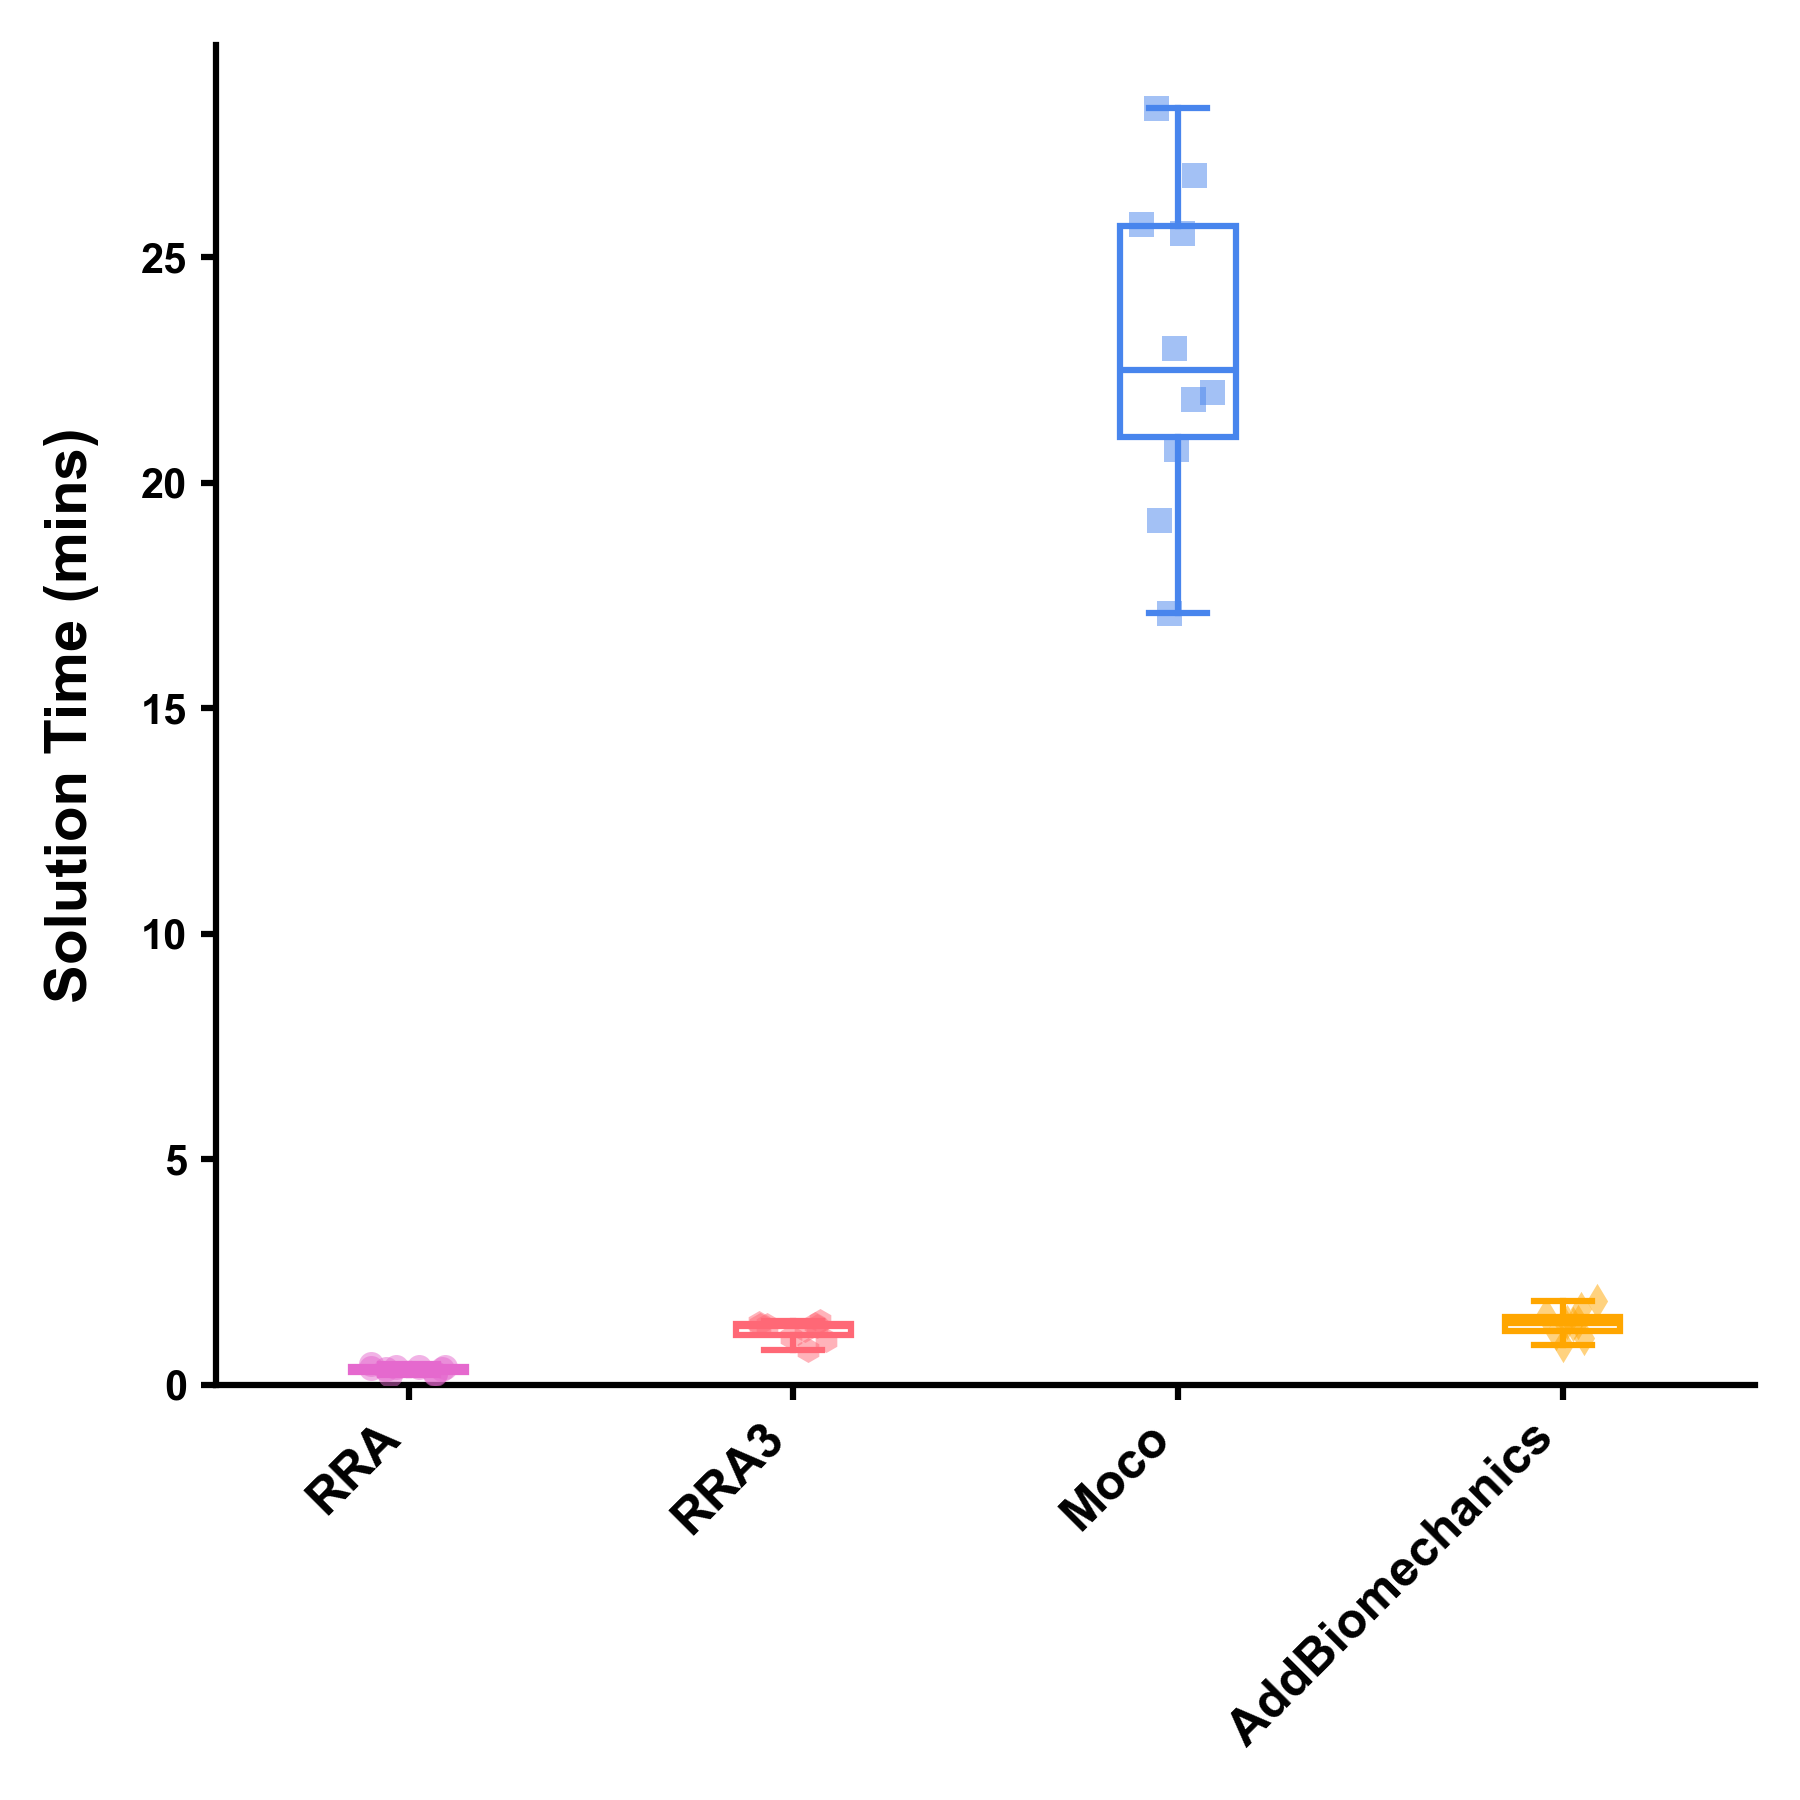
\includegraphics[width=0.75\linewidth]{../results/HamnerDelpDataset/figures/averageSolutionTimes} 

}

\caption{Solution times (in minutes) for processing a gait cycle using the Residual Reduction Algorithm (RRA — Purple), Iterative Residual Reduction Algorithm  (RRA3 — Pink), MocoTracking (Moco — Blue), and AddBiomechanics (Gold) approaches. Horizontal lines within boxes equate to the median value, boxes indicate the 25$^{th}$ to 75$^{th}$ percentile, and whiskers indicate the range. Average solution times for each participants three gait cycles are displayed as points.}\label{fig:computationalTimes}
\end{figure}

\hypertarget{residual-forces}{%
\subsection{Residual Forces}\label{residual-forces}}

Average and peak residual forces (see Figure \ref{fig:residualForces})
were, on average, highest in the RRA approach (mean ± SD average
residuals of 15.28 ± 3.20, 16.16 ± 5.52 and 13.96 ± 2.05 for FX, FY and
FZ, respectively; mean ± SD peak residuals of 44.87 ± 6.63, 43.91 ±
12.05 and 43.55 ± 8.12 for FX, FY and FZ, respectively) followed by the
RRA3 (average residuals of 9.15 ± 1.77, 8.96 ± 2.65 and 8.68 ± 1.58 for
FX, FY and FZ, respectively; peak residuals of 26.78 ± 4.15, 27.63 ±
7.25 and 29.16 ± 8.18 for FX, FY and FZ, respectively) and
\emph{AddBiomechanics} (average residuals of 8.11 ± 21.35, 16.35 ± 42.53
and 7.33 ± 19.52 for FX, FY and FZ, respectively; peak residuals of
40.61 ± 76.45, 62.65 ± 111.19 and 25.39 ± 52.70 for FX, FY and FZ,
respectively) approaches. In almost all cases, the \emph{MocoTrack}
approach recorded the lowest average and peak residual forces (average
residuals of 0.14 ± 0.20, 0.33 ± 0.47 and 0.13 ± 0.13 for FX, FY and FZ,
respectively; peak residuals of 0.32 ± 0.46, 0.66 ± 0.97 and 0.34 ± 0.37
for FX, FY and FZ, respectively). The RRA, RRA3 and \emph{MocoTrack}
approaches were able to achieve acceptable average and peak residual
forces according to the threshold proposed by Hicks et al.
\citep{Hicks2015} on average across all participants gait cycles. The
\emph{AddBiomechanics} approach also subceeded this threshold for the
majority of participants, with the exception of one or two cases.

\begin{figure}

{\centering 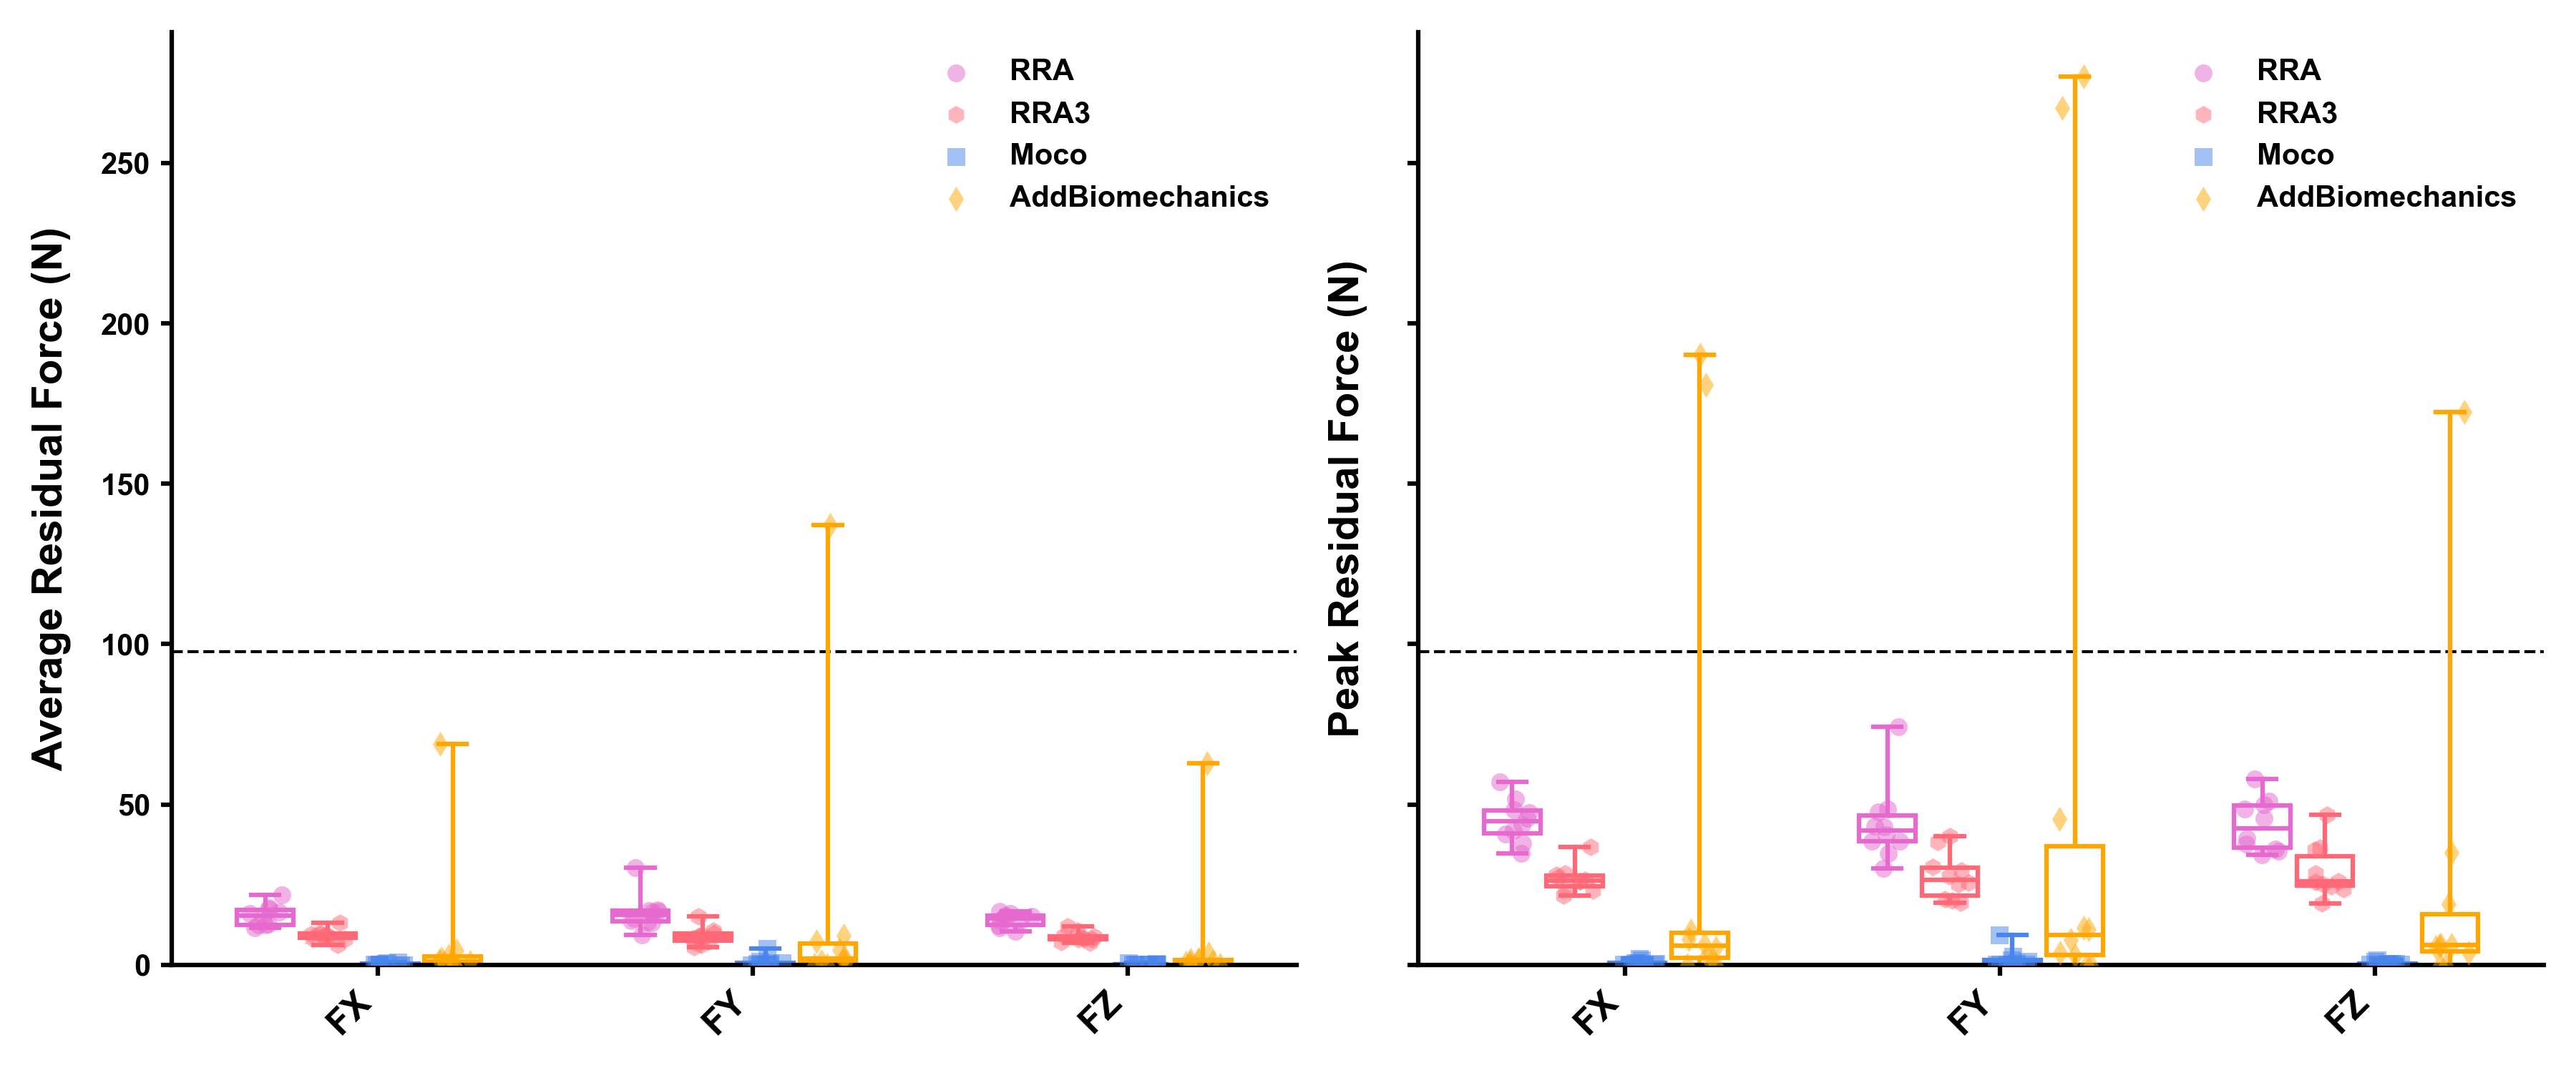
\includegraphics[width=1\linewidth]{../results/HamnerDelpDataset/figures/residualForces} 

}

\caption{Average (left panel) and peak (right panel) residual forces (in Newtons [N]) for gait cycles processed using the Residual Reduction Algorithm (RRA — Purple), Iterative Residual Reduction Algorithm  (RRA3 — Pink), MocoTracking (Moco — Blue), and AddBiomechanics (Gold) approaches. Horizontal lines within boxes equate to the median value, boxes indicate the 25$^{th}$ to 75$^{th}$ percentile, and whiskers indicate the range. Average residual forces for each participants three gait cycles are displayed as points. The black dashed line represents the proposed acceptable threshold for residual forces.}\label{fig:residualForces}
\end{figure}

\hypertarget{residual-moments}{%
\subsection{Residual Moments}\label{residual-moments}}

Average and peak residual moments (see Figure \ref{fig:residualMoments})
were typically highest in the RRA (mean ± SD average residuals of 26.72
± 5.13, 24.57 ± 2.89 and 43.36 ± 7.90 for MX, MY and MZ, respectively;
mean ± SD peak residuals of 83.02 ± 19.02, 70.84 ± 10.88 and 129.75 ±
20.66 for MX, MY and MZ, respectively) and \emph{AddBiomechanics}
(average residuals of 27.29 ± 6.01, 16.07 ± 4.91 and 27.84 ± 6.81 for
MX, MY and MZ, respectively; peak residuals of 79.94 ± 15.63, 43.00 ±
11.69 and 90.56 ± 20.83 for MX, MY and MZ, respectively) approaches,
followed by the RRA3 approach (average residuals of 12.71 ± 3.17, 18.86
± 2.50 and 24.59 ± 4.90 for MX, MY and MZ, respectively; peak residuals
of 44.77 ± 11.25, 57.96 ± 18.42 and 74.63 ± 12.12 for MX, MY and MZ,
respectively). The \emph{MocoTrack} approach recorded the lowest average
and peak residual moments (average residuals of 0.33 ± 0.30, 0.85 ± 0.54
and 0.40 ± 0.41 for MX, MY and MZ, respectively; peak residuals of 0.90
± 0.79, 2.30 ± 1.72 and 0.95 ± 0.91 for MX, MY and MZ, respectively) in
all participants. Only the \emph{MocoTrack} approach was able to
consistently achieve acceptable average and peak residual moments
according to the threshold proposed by Hicks et al. \citep{Hicks2015}
across all participants gait cycles. Average residual moments from the
RRA, RRA3 and \emph{AddBiomechanics} approaches rarely subceeded, while
the peak residual moments were always above this threshold.

\begin{figure}

{\centering 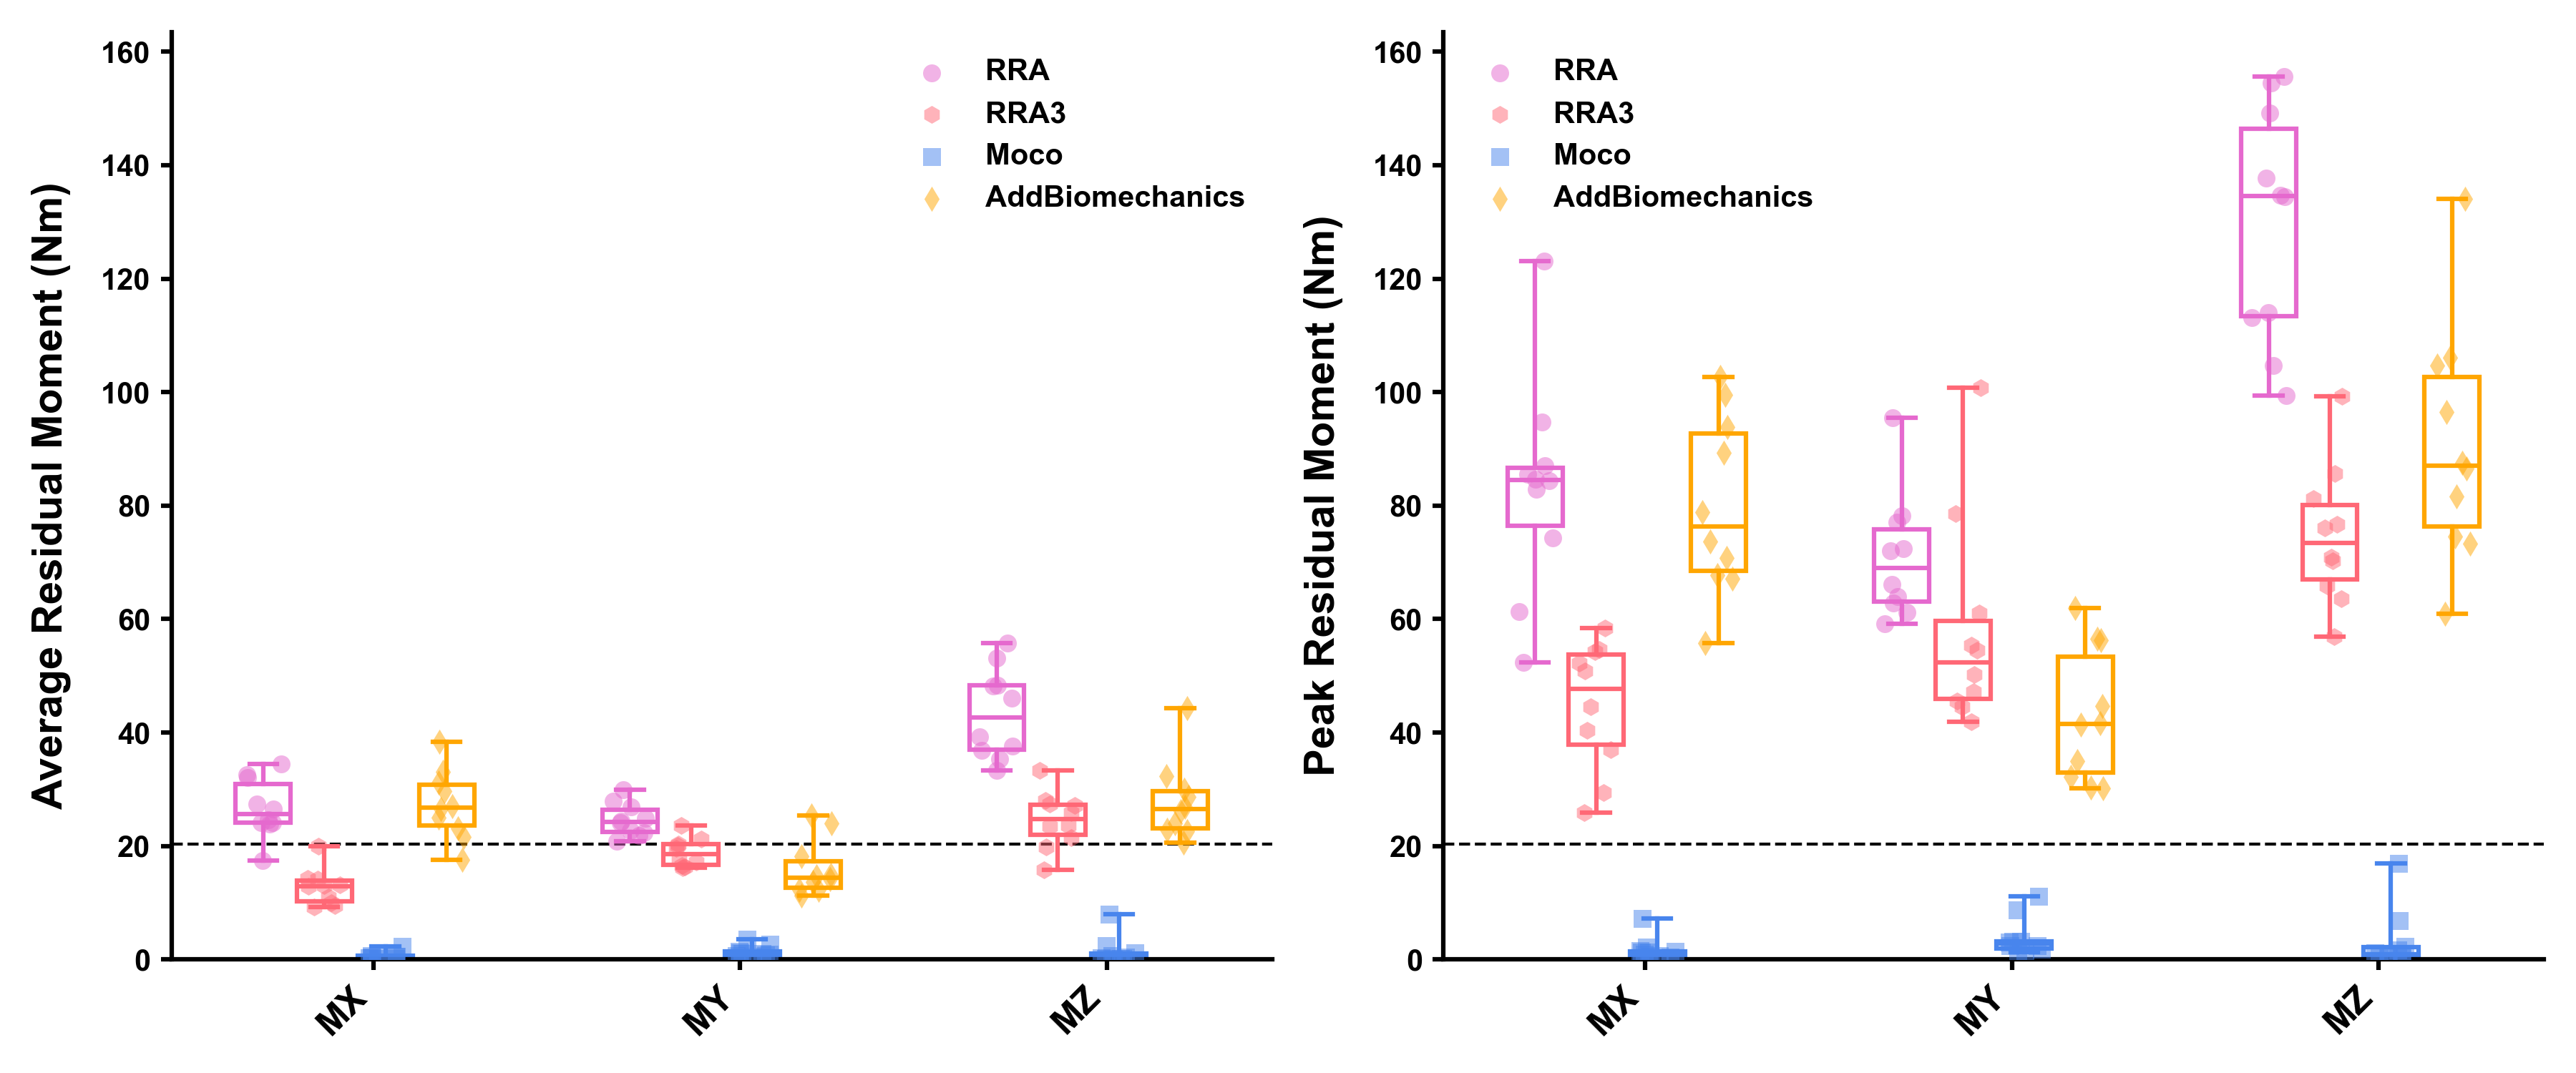
\includegraphics[width=1\linewidth]{../results/HamnerDelpDataset/figures/residualMoments} 

}

\caption{Average (left panel) and peak (right panel) residual moments (in Newton-Metres [Nm]) for gait cycles processed using the Residual Reduction Algorithm (RRA — Purple), Iterative Residual Reduction Algorithm  (RRA3 — Pink), MocoTracking (Moco — Blue), and AddBiomechanics (Gold) approaches. Horizontal lines within boxes equate to the median value, boxes indicate the 25$^{th}$ to 75$^{th}$ percentile, and whiskers indicate the range. Average residual moments for each participants three gait cycles are displayed as points. The black dashed line represents the proposed acceptable threshold for residual moments.}\label{fig:residualMoments}
\end{figure}

\hypertarget{joint-kinematics}{%
\subsection{Joint Kinematics}\label{joint-kinematics}}

Average joint kinematics were qualitatively similar across approaches
for the majority of joint coordinates (see Figure
\ref{fig:jointKinematics}). The greatest kinematic variations were for
pelvic tilt, hip adduction/abduction and internal/external rotation, and
ankle plantarflexion/dorsiflexion between \emph{AddBiomechanics} and the
other approaches; and for upper body kinematics (i.e.~shoulder and elbow
joint angles) between \emph{MocoTrack} and the other approaches.

\begin{figure}

{\centering 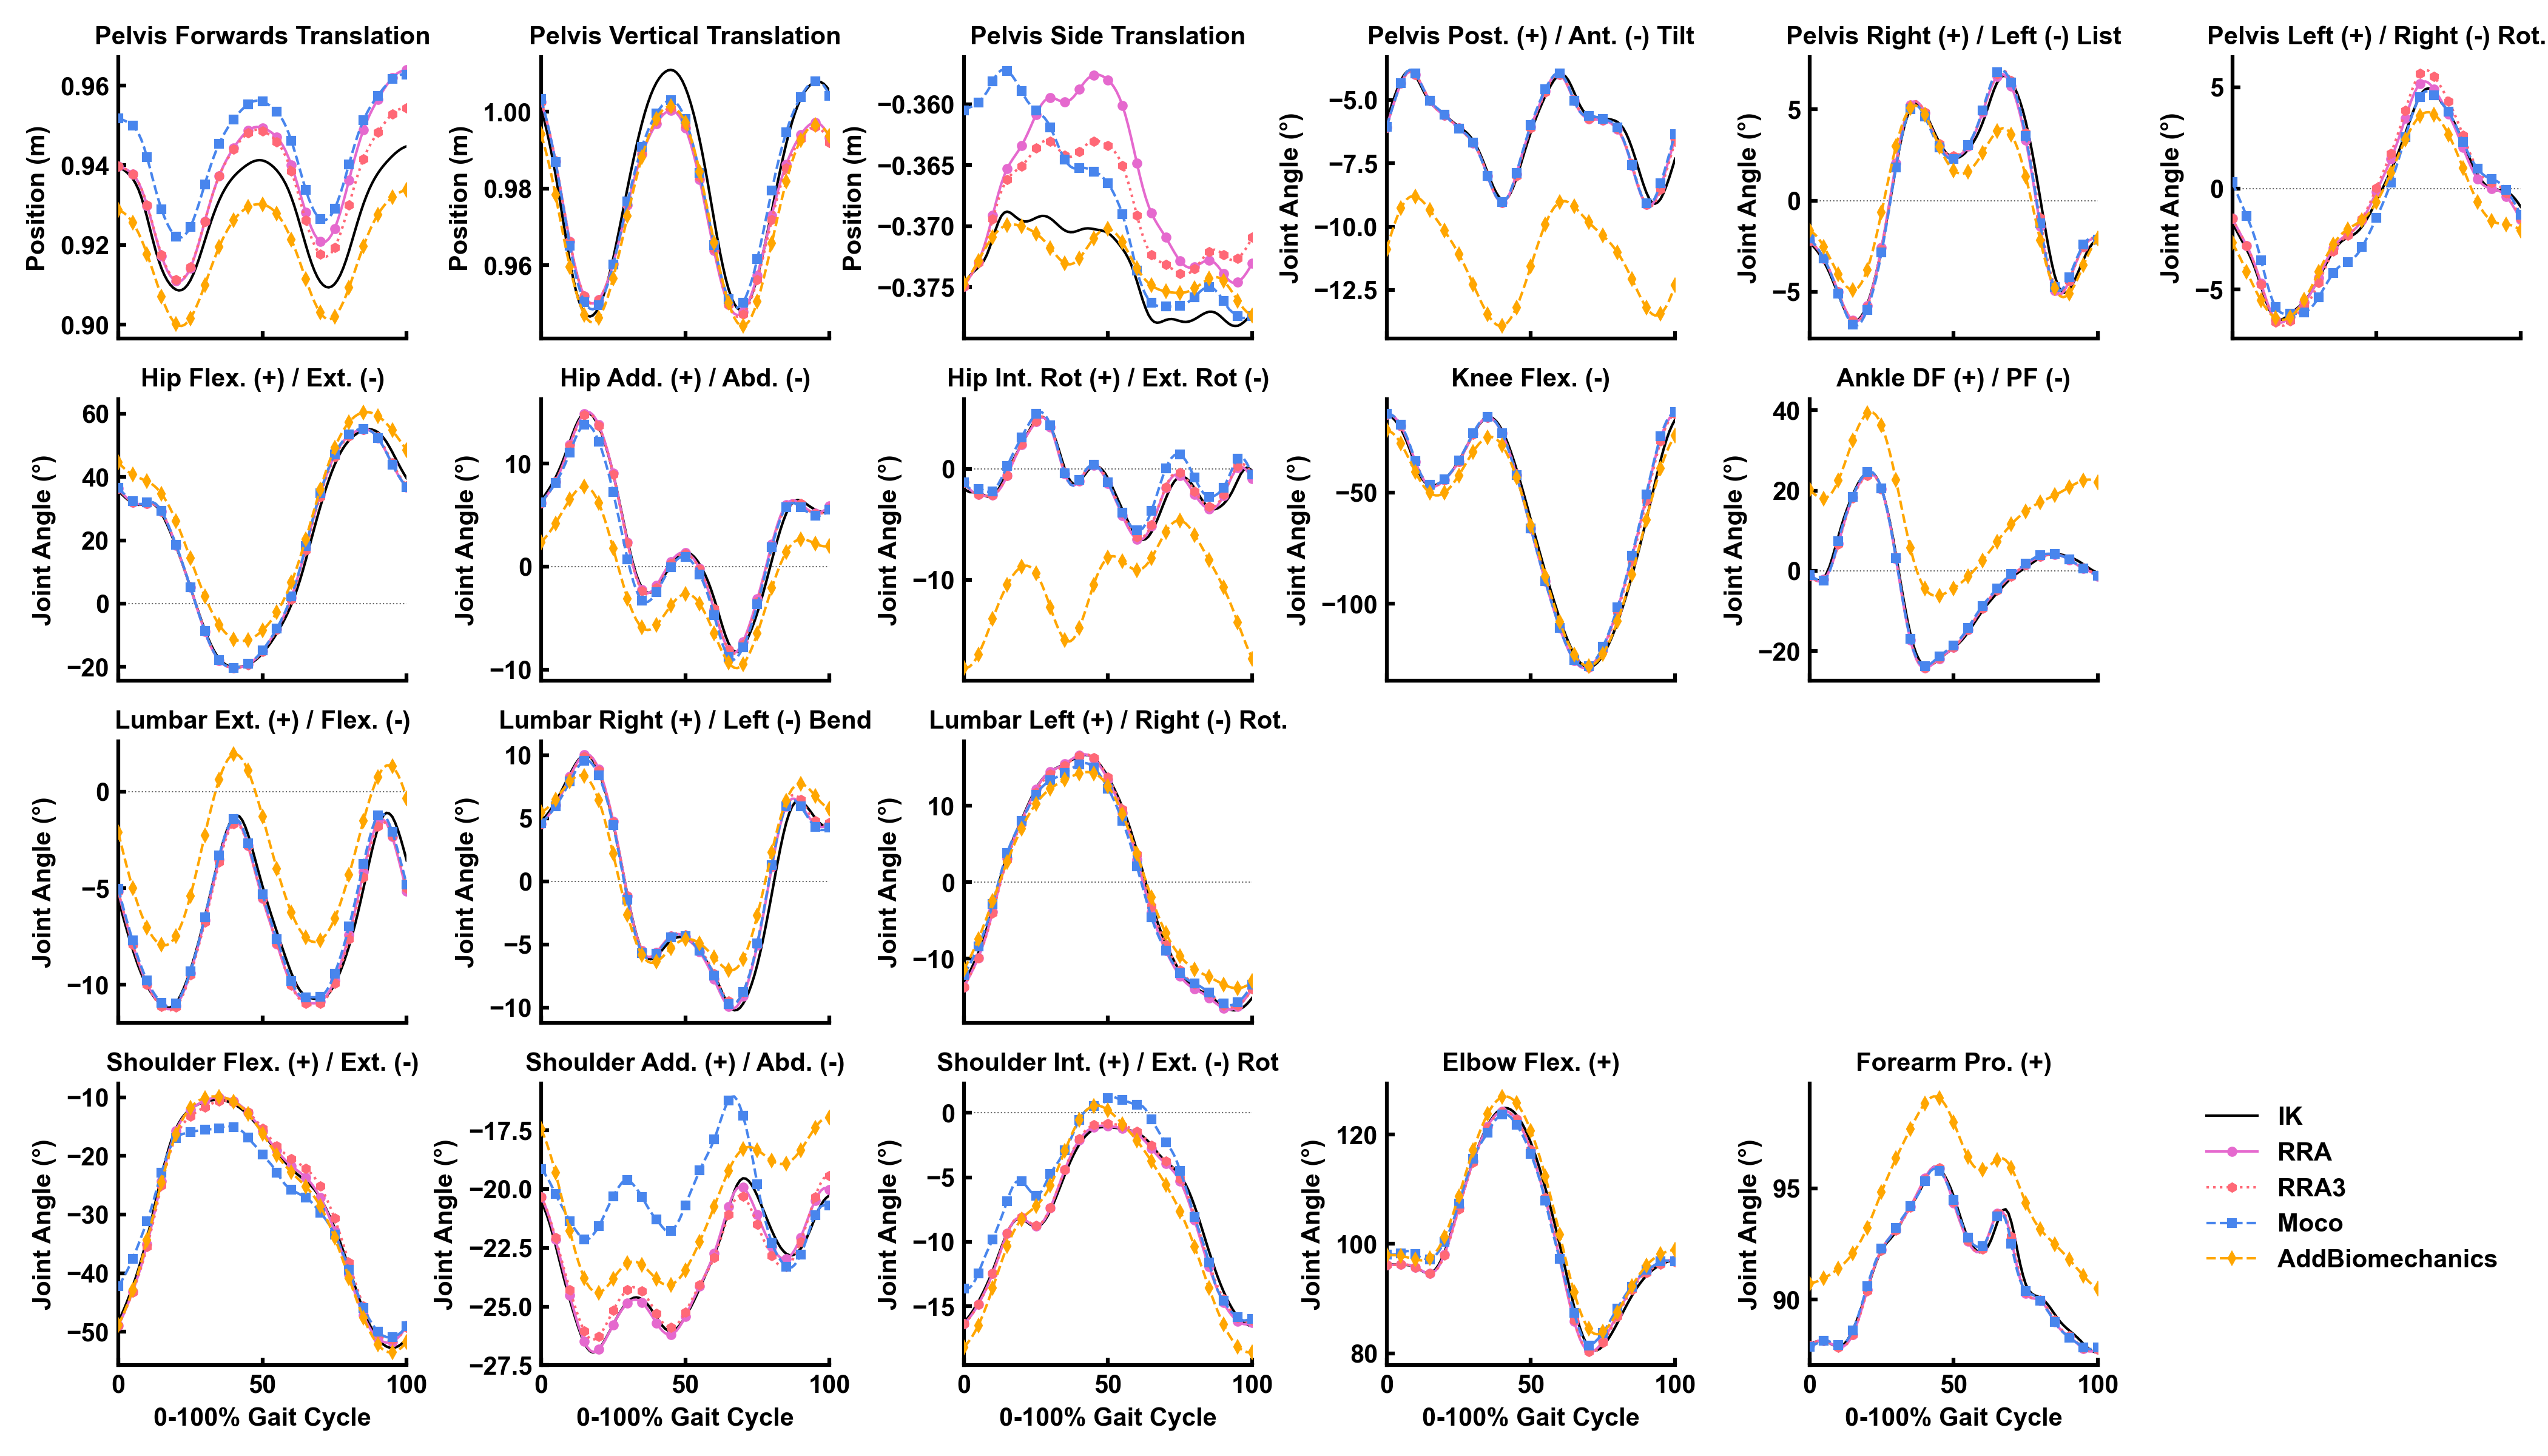
\includegraphics[width=1\linewidth]{../results/HamnerDelpDataset/figures/meanKinematics} 

}

\caption{Mean (solid lines) ± standard deviation (shaded areas) of joint kinematics (in degrees) for gait cycles processed using Inverse Kinematics (IK), Residual Reduction Algorithm (RRA — Purple), Iterative Residual Reduction Algorithm  (RRA3 — Pink), MocoTracking (Moco — Blue), and AddBiomechanics (Gold) approaches.}\label{fig:jointKinematics}
\end{figure}

\hypertarget{joint-kinetics}{%
\subsection{Joint Kinetics}\label{joint-kinetics}}

Average joint kinetics were qualitatively similar across approaches for
all joint moments, with the exception of significant noise appearing in
the \emph{MocoTrack} signals (see Figure \ref{fig:jointKinetics}).

\begin{figure}

{\centering 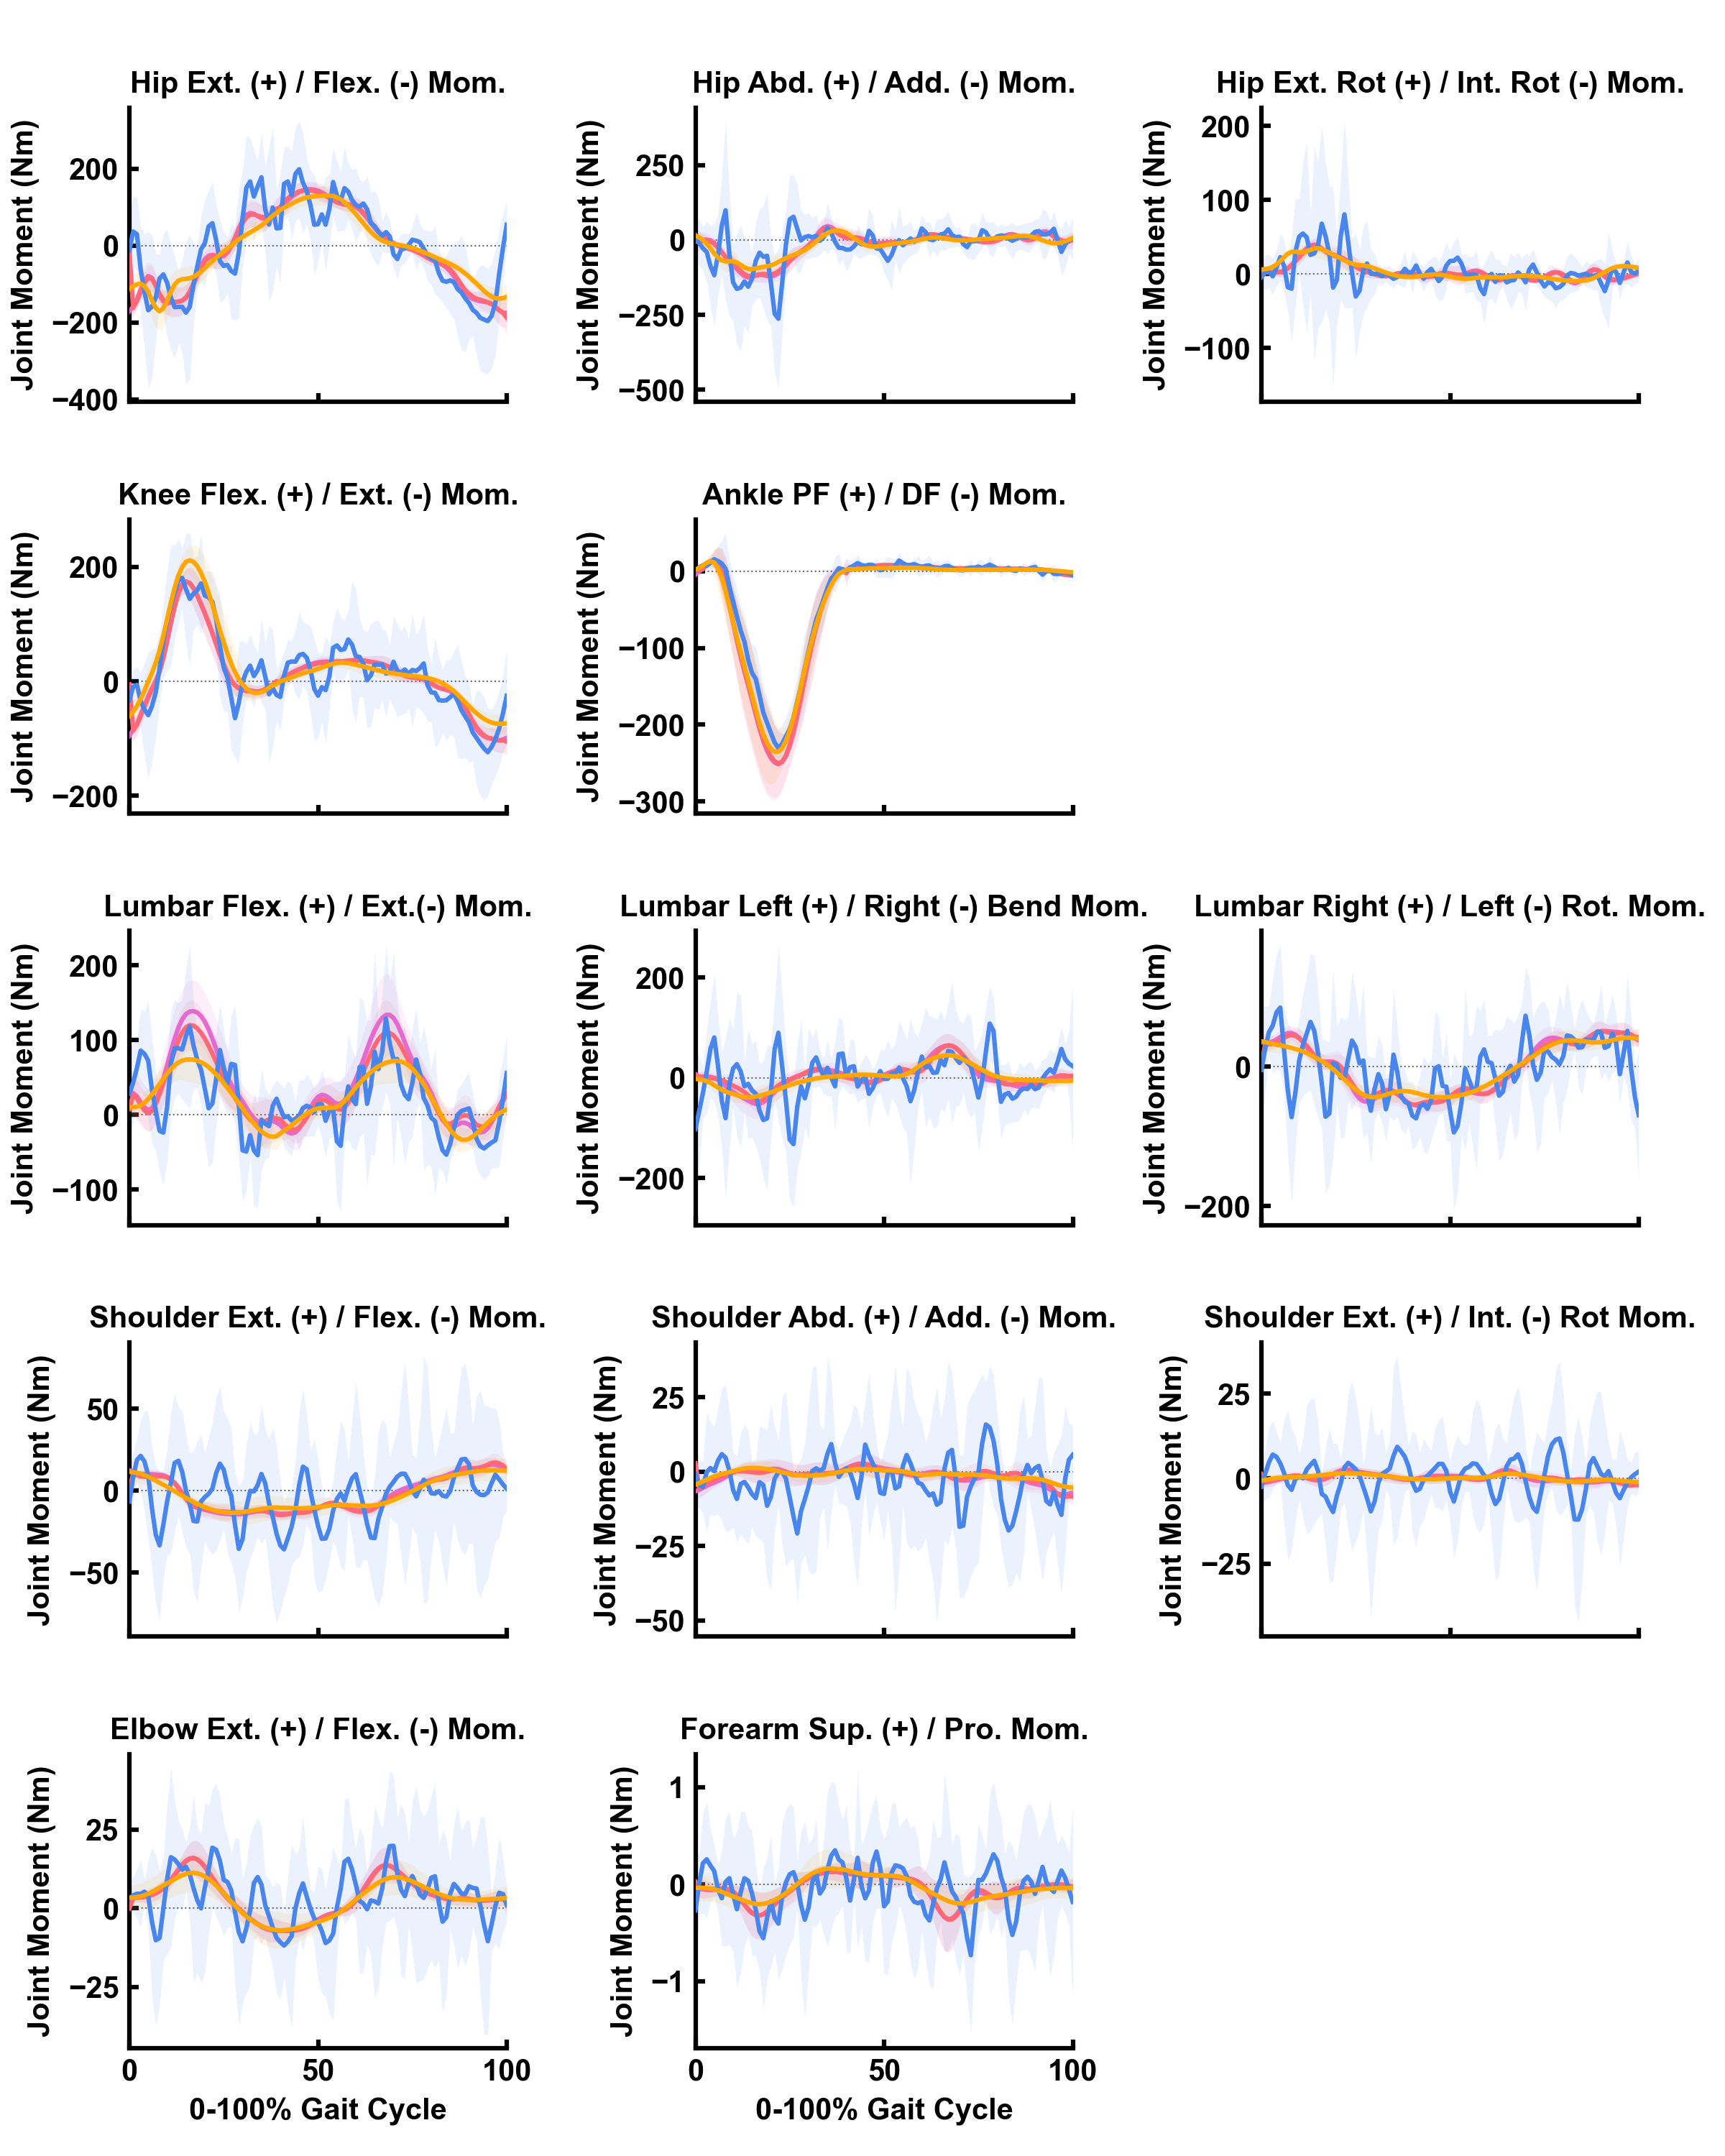
\includegraphics[width=1\linewidth]{../results/HamnerDelpDataset/figures/meanKinetics} 

}

\caption{Mean (solid lines) ± standard deviation (shaded areas) of joint moments (in Newton-Metres [Nm]) for gait cycles processed using the Residual Reduction Algorithm (RRA — Purple), Iterative Residual Reduction Algorithm  (RRA3 — Pink), MocoTracking (Moco — Blue), and AddBiomechanics (Gold) approaches.}\label{fig:jointKinetics}
\end{figure}

\hypertarget{discussion}{%
\section{Discussion}\label{discussion}}

Dynamic inconsistencies in simulations of human running can lead to
unrealistic musculoskeletal model outputs (e.g.~joint moments, muscle
forces). Minimising the residual forces and moments at a models root
segment is subsequently a recommended step within simulation pipelines
\citep{Delp2007, Hicks2015}. OpenSim --- likely the most widely used
musculoskeletal modelling and simulation software --- now offers a
variety of approaches applicable to residual reduction, yet these have
never undergone a comprehensive comparison. This study aimed to compare
the computational times, resultant residual forces and moments, and
output joint kinematics and kinetics of different residual reduction
approaches --- or in more extravagant terms, set out on a quest for
dynamic consistency in simulations of human running. A clear
computational cost to residual reduction trade-off was identified, where
approaches that required longer computational times were more effective
at minimising residual forces and moments. In the majority of
simulations, all approaches were able to reduce residual forces below
recommended thresholds. However, only the \emph{MocoTrack} approach was
able to consistently achieve acceptable levels for residual moments.
Minimal qualitative differences were observed in the resultant joint
kinematics, with the exception of the \emph{AddBiomechanics} and
\emph{MocoTrack} approaches producing variable lower and upper body
kinematics, respectively, versus the remaining approaches. Joint
kinetics were qualitatively similar between approaches despite the
\emph{MocoTrack} approach generating much noisier signals.

~

The present study revealed a clear trade-off between computational time
and the capacity to reduce residual forces and moments. \emph{MocoTrack}
was by far the best and most consistent approach for reducing residuals,
achieving near-zero levels (see Figures \ref{fig:residualForces} and
\ref{fig:residualMoments}), and was the only approach that consistently
reduced both residual forces and moments below recommended thresholds
\citep{Hicks2015}. However, the \emph{MocoTrack} approach took
approximately 4-60 times longer than all others on average. Although
\emph{MocoTrack} had the highest computational times in the present
study, the approximate 15-30 minute time-range substantially outperforms
previous efforts \citep{Samaan2016, Sturdy2022} to optimise the RRA
process. It is likely that studies with a smaller sample (i.e.~lower
participant numbers and gait cycles to process) would be able to
implement the \emph{MocoTrack} approach, yet substantially larger
studies may need to consider the longer computational times. The lower
computational time of the \emph{AddBiomechanics} approach must also be
considered in the context of how it was assessed. An estimate of the
\emph{AddBiomechanics} processing time was taken from the processing
logs in the application --- and hence does not include the time taken to
upload the data, how long the data was queued on the computing cluster,
and the time taken to download the processed data. Uploads and downloads
typically took less than a few minutes, while the cluster queue times
were more variable and hence could add up for studies with large
samples. Alternatively, users could consider these additional time costs
as being offset against the unique time-saving aspects of using
\emph{AddBiomechanics} (e.g.~outsourcing data processing, and removing
the need for static trials and model scaling).

~

The joint kinematics produced by all approaches were, for the most part,
qualitatively similar to one another (see Figure
\ref{fig:jointKinematics}). The major exceptions were the pelvic tilt,
frontal and transverse plane hip, and sagittal plane ankle angles from
\emph{AddBiomechanics} versus other approaches; and the shoulder and
elbow joint angles from \emph{MocoTrack} versus other approaches. While
visualising the overall average motion demonstrates the relative
whole-body consistency across approaches (see Figure
\ref{fig:overallMotion}), the specific differences at certain joints are
also evident. The potential for variation in joint kinematics highlights
the need to consider the residual reduction approach used when comparing
results across studies, particularly for the joint angles that more
largely varied. It is difficult to determine which approach achieved the
most `accurate' joint kinematics given the lack of a gold-standard
measure to evaluate against. The inverse kinematic (IK) and
\emph{AddBiomechanics} joint kinematic solutions are derived by tracking
experimental marker data, and therefore marker tracking error is a
potential measure of accuracy for these approaches. However, marker
error may not be a valid comparison to the RRA and \emph{MocoTrack}
approaches. The joint kinematics for RRA/RRA3 and \emph{MocoTrack} were
derived from tracking the IK results, and hence any initial marker
errors in the IK data would likely propagate forwards and potentially
increase in these solutions. Directly tracking marker data (instead of
joint coordinates) alongside GRFs is a potential option within the
\emph{MocoTrack} framework \citep{Nitschke2023}. Using a marker-tracking
approach could also be valid in reducing residuals in running
simulations and provide a more accurate comparison to the other
marker-based approaches (i.e.~IK and \emph{AddBiomechanics}), however
was not considered in the present study.

\begin{figure}

{\centering 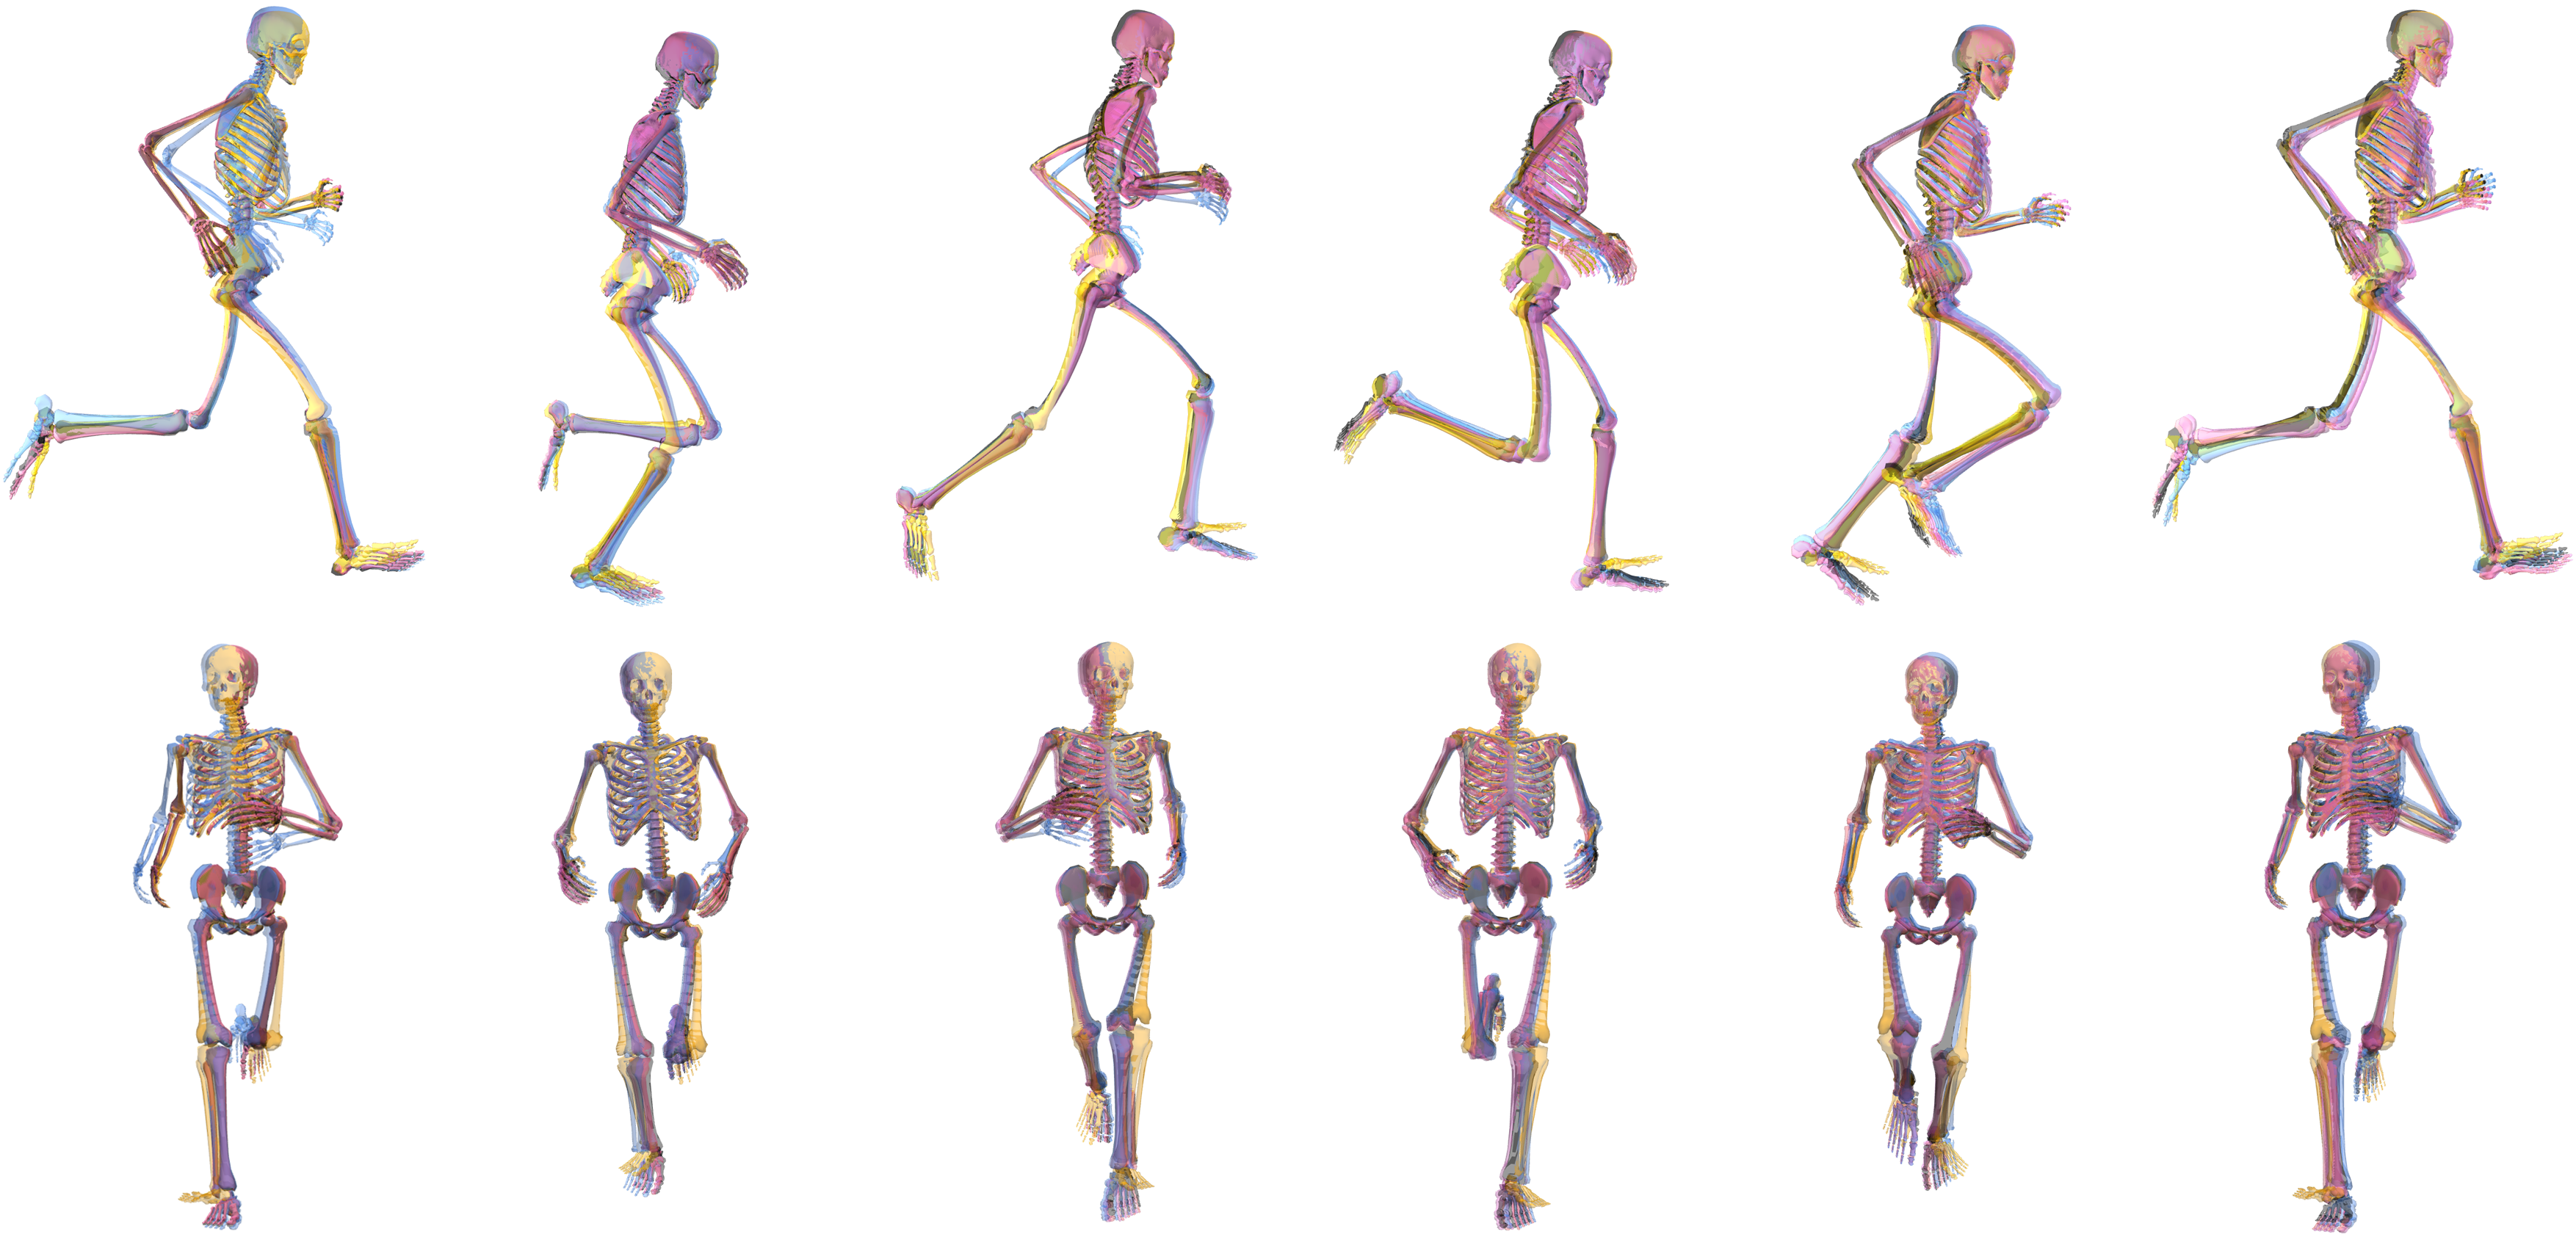
\includegraphics[width=0.9\linewidth]{../results/HamnerDelpDataset/figures/meanKinematics_gaitCycleVisualised_combinedPlanes} 

}

\caption{Group average joint motion at from the Residual Reduction Algorithm (RRA — Purple), Iterative Residual Reduction Algorithm  (RRA3 — Pink), MocoTracking (Moco — Blue), and AddBiomechanics (Gold) approaches in the sagittal and frontal planes.}\label{fig:overallMotion}
\end{figure}

~

Similar to joint kinematics, the joint kinetics produced by all
approaches were qualitatively similar (see Figure
\ref{fig:jointKinetics}). However, the joint kinetics from
\emph{MocoTrack} were substantially noisier than those from all other
approaches. Using a smaller time-step in torque-driven simulations can
generate noisier signals from actuators driving joint motions, given the
larger gap between sample points potentially requiring more abrupt
shifts in the joint moments required. A smaller time-step was selected
for the \emph{MocoTrack} (i.e.~0.01s) versus RRA/RRA3 approaches
(i.e.~0.0001s) in the present study for practical reasons, while the
time-step in the \emph{AddBiomechanics} approach is automatically
determined based on the sampling rate of marker data (that being 0.01s
in the dataset used). If the smaller time-step was a valid explanation
for the noisier joint moments from \emph{MocoTrack}, it could be assumed
that the same phenomenon would present in the \emph{AddBiomechanics}
outputs --- yet this was not the case. A more likely explanation is that
the noise captured in the joint kinetics of the \emph{MocoTrack}
solution is simply being captured elsewhere in the other approaches.
This begs the question, where did the noise go? The residual forces and
moments that remained in the RRA, RRA3 and \emph{AddBiomechanics}
solutions were inherently noisy (see Figure
\ref{fig:sampleSubjectResiduals} for an individual participant example),
and perhaps offer a reason for why these approaches were able to achieve
much smoother joint kinetic signals. The musculoskeletal models used in
the present study were rigid in nature, which subsequently ignores soft
tissue motion in the dynamics analyses and may offer an explanation for
the lingering noise present in the simulations. Combining residual
reduction approaches with more complex models (e.g.~that include
wobbling masses) may better capture joint dynamics while accounting for
soft tissue motion \citep{Masters2022}.

\begin{figure}

{\centering 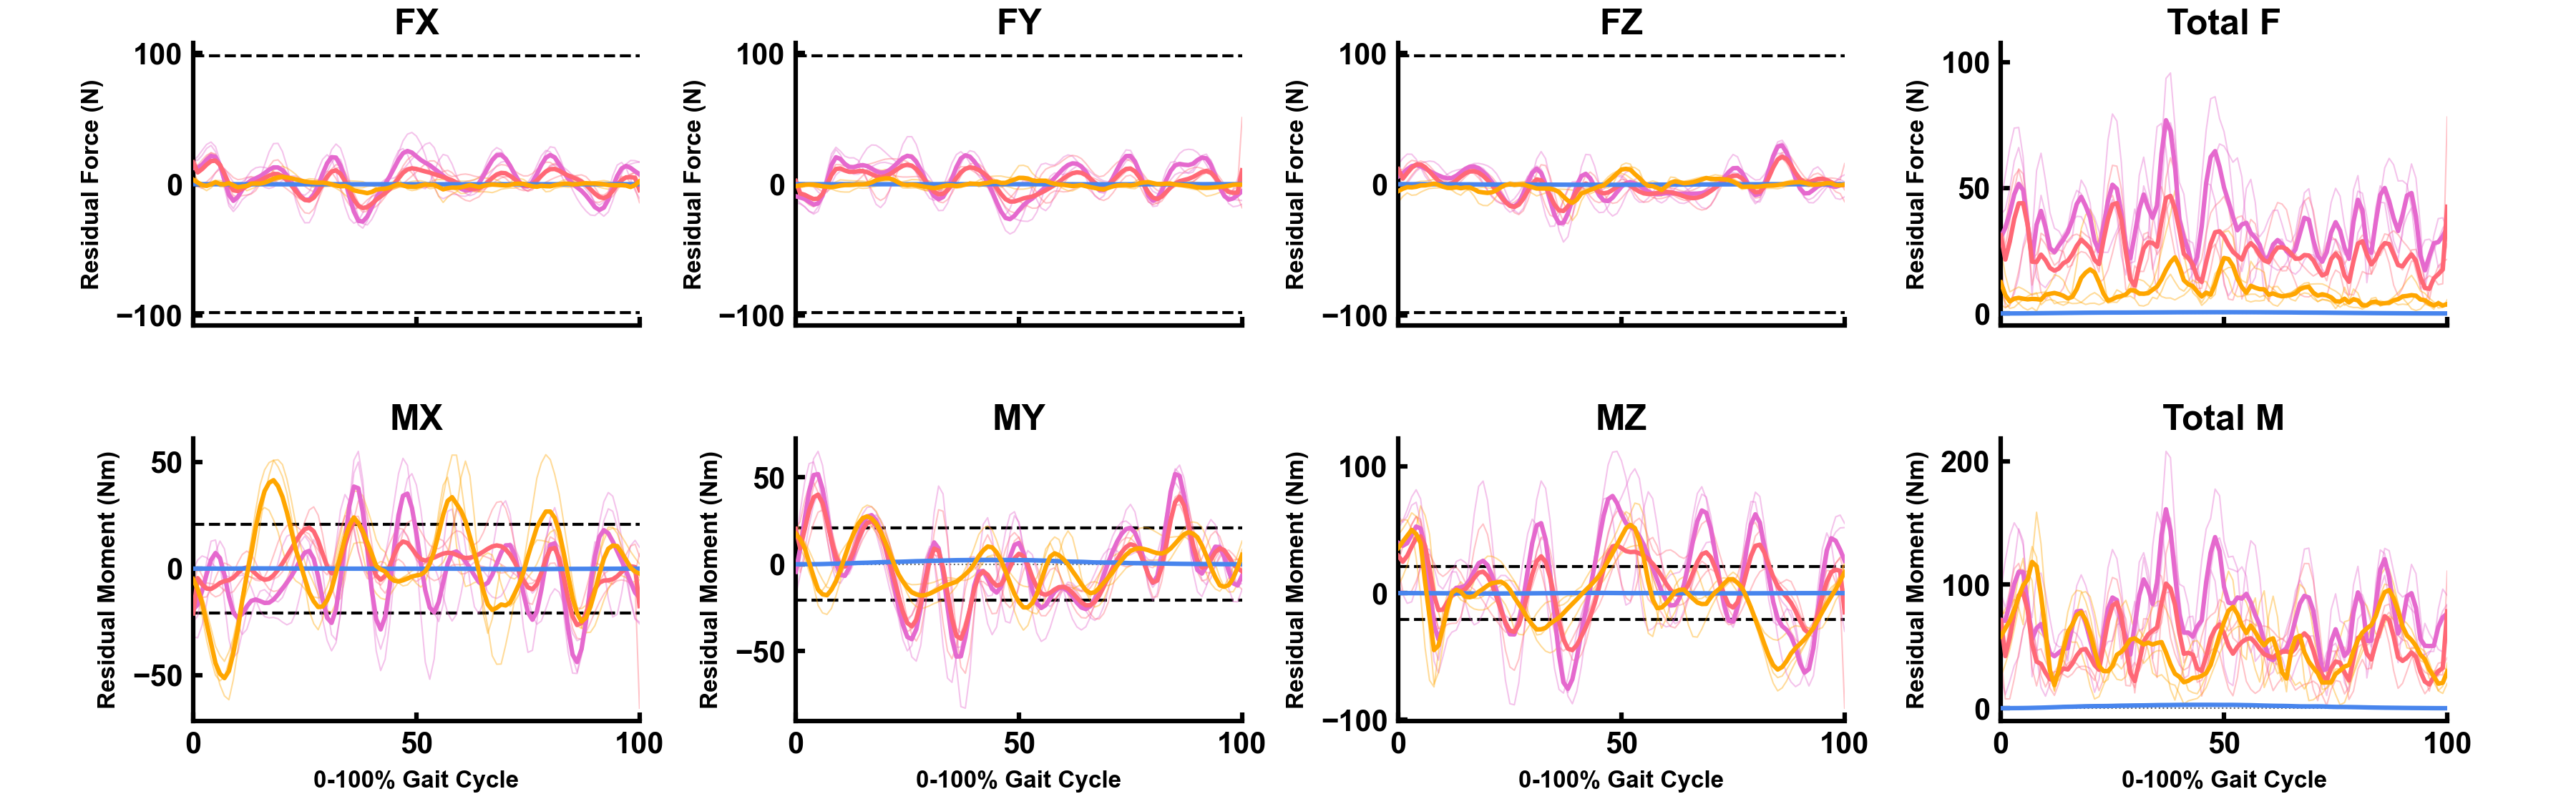
\includegraphics[width=1\linewidth]{../results/HamnerDelpDataset/figures/subject01_run5_residualsComparison} 

}

\caption{Average (thick line) and individual gait cycle (thin lines) residual forces (FX, FY, FZ and Total F) and moments (MX, MY, MZ and Total M) for the Residual Reduction Algorithm (RRA — Purple), Iterative Residual Reduction Algorithm  (RRA3 — Pink), MocoTracking (Moco — Blue), and AddBiomechanics (Gold) approaches from a single participant example.}\label{fig:sampleSubjectResiduals}
\end{figure}

~

For the sake of complete honesty, very little effort went into selection
of the input parameters and settings used in the various approaches.
Where possible, the parameters used in the original work of Hamner and
Delp \citep{Hamner2013} were replicated (i.e.~tracking task weights and
torque actuator settings in RRA) and reproduced in other approaches
(i.e.~RRA3 and \emph{MocoTrack}). There are few objective
recommendations for selecting these settings, hence the replication of
the original studies \citep{Hamner2013} approach aimed to eliminate any
additional subjectivity being added. Similarly, the default parameters
in the \emph{AddBiomechanics} application (e.g.~the weight of residuals
in the main optimisation) were not altered in any way. The results from
the present study should therefore be considered with respect to the
settings and parameters used for each approach. Past work has
demonstrated that optimising the settings within residual reduction
approaches can improve the dynamic consistency of the simulation,
typically at the cost of additional computational time used to identify
the optimised settings \citep{Samaan2016, Sturdy2022}. Therefore, there
may be room for improvement within the residual forces and moments
achieved in the present study --- yet users must consider the added
computational time to deduce these. The time-frames and residuals
reported in previous work optimising the RRA approach
\citep{Samaan2016, Sturdy2022} still exceed those of the best performing
\emph{MocoTrack} approach in the present study (i.e.~\textasciitilde20
minutes for near-zero residuals with \emph{MocoTrack}) --- highlighting
the effectiveness of this method even with minimal consideration of the
input settings and parameters.

~

While the findings of the present study could support a broad
recommendation for the \emph{MocoTrack} approach, there is a practical
user-based element to consider with respect to wide-spread adoption. At
present, OpenSim's Moco tools are only accessible via C++, MATLAB or
Python scripting. In contrast, the RRA approaches can be accessed in
this way plus via the graphical user interface (GUI); while the
\emph{AddBiomechanics} approach is accessible via a simple-to-use web
application. Therefore, only OpenSim users with appropriate scripting
knowledge and skills could theoretically implement the \emph{MocoTrack}
approach. There is no information as to what proportion of the OpenSim
user base would fit this description, but it is unlikely to be everyone.
The analysis code (in Python) from the present study is publicly
available (see the
\href{https://simtk.org/projects/dynamic-quest}{associated SimTK project
page} at https://simtk.org/projects/dynamic-quest) to support
implementation of similar approaches. However, integration of the Moco
suite of tools into the OpenSim GUI would likely support further use.

\hypertarget{limitations}{%
\subsection{Limitations}\label{limitations}}

The findings from this study must be considered within the scope of the
work. Only treadmill running at a single speed, in a healthy population
and using a relatively small sample size (\emph{n} = 10) was examined.
The singular fastest speed in the dataset (i.e.~5.0
m·s\textsuperscript{-1}) was chosen given the expected higher forces and
accelerations having the potential to generate larger residual forces
and moments. The various residual reduction approaches examined likely
have a similar ability across different running speeds, however the
results from the present study cannot confirm or refute this. It is
possible that the magnitude of difference in residuals between the
approaches could reduce at slower running speeds or in slower gait tasks
(e.g.~walking) --- potentially making some of the lesser performing
approaches more valid in these contexts. Similarly, there may be some
variation in the success of the residual reduction approaches when
examining overground instead of treadmill running. Given a single gait
cycle was processed for most residual reduction approaches, it is
expected that any difference between these running modalities would be
minimal. The \emph{AddBiomechanics} approach, however, may be the most
affected given the whole-trial processing and potentially limited number
of gait cycles that could be captured in a single overground trial.
Lastly, performance of the residual reduction approaches may vary when
examining altered gait in clinical populations (e.g.~crouch gait or
toe-walking in cerebral palsy).

\hypertarget{conclusions}{%
\section{Conclusions}\label{conclusions}}

This study set out on a quest for dynamic consistency in simulations of
human running by examining different residual reduction approaches
(single and iterative RRA, \emph{MocoTrack} and \emph{AddBiomechanics})
available to OpenSim users. A computational time to residual reduction
trade-off was identified, where approaches that took longer were more
effective in reducing residual forces and moments. \emph{MocoTrack} was
the most consistent and best performing approach for reducing residuals
to near-zero levels, however required substantially longer computational
times and produced noisier joint kinetic signals. Joint kinematics were
mostly similar across the residual reduction approaches, however
specific joint angle variations occurred with certain approaches. The
findings from the present study provide a comprehensive analysis of the
simulation outputs when using different residual reduction approaches in
OpenSim, providing users with evidence to inform decision-making at the
residual reduction step of their modelling and simulation workflow when
analysing human running.

\hypertarget{acknowledgements}{%
\section{Acknowledgements}\label{acknowledgements}}

Thanks must go to those who asked questions and discussed this work at
the 2023 International Symposium on Computer Simulation in Biomechanics
(organised by the Technical Group on Computer Simulation of the
International Society of Biomechanics) --- with special thanks to Ajay
Seth for proposing a new, more extravagant title.

\newpage

\bibliography{references.bib}


\end{document}
